% !TeX spellcheck = en_GB

% ------------------------------- %

\begin{frame}{\dots dataset}

\begin{columns}[T]
\begin{column}{0.5\textwidth}

\end{column}
\begin{column}{0.5\textwidth}
Binary classification task $\mathcal{Y}\in\set{0,1}$% (disease -- no disease)

Class distribution: 0.49 -- 0.51

Approaches
\begin{itemize}
	\item Decision tree
	\item Random forest
	\item AdaBoost
	\item Ridge logistic regression
	\item Super learner
\end{itemize}
\end{column}
\end{columns}

\end{frame}

% ------------------------------- %

\begin{frame}[fragile]{Random forest}

\begin{columns}[T]
\begin{column}{0.65\textwidth}
\begin{figure}
\centering
\vspace*{-0.5em}\begin{tikzpicture}
	%draw,ellipse,fill=red!20,minimum height=2em,text centered,font=\sffamily\small
	\tikzset{help lines/.append style=pink}
%	\draw [help lines] (-1,-4) grid (7,2); \node[draw,circle,fill=red] at (0,0) {};
	
	\node[cloud3] (b1) at (0,0) {$\pi_1, m_1$};
	\node[cloud3] (b2) at ($(b1)+(1.8,0)$) {$\pi_2, m_2$};
	\node[cloud3] (B) at ($(b2)+(3,0)$) {$\pi_B, m_B$};
	\draw[-,dotted,very thick] (b1) to (b2);
	\draw[-,dotted,very thick] (b2) to (B);
	
	\node[] (T1) at ($(b1)+(0,-1.3)$) {$T_1$};
	\node[] (T2) at ($(b2)+(0,-1.3)$) {$T_2$};
	\node[] (TB) at ($(B)+(0,-1.3)$) {$T_B$};
	\draw[-stealth] ($(b1.south)+(0,-0.15)$) to (T1);
	\draw[-stealth] ($(b2.south)+(0,-0.15)$) to (T2);
	\draw[-stealth] ($(B.south)+(0,-0.15)$) to (TB);
	
	\begingroup\linespread{0.9}
	\node[font=\footnotesize,text width=4em,centered,text centered,inner sep=0pt] (m) at (3.3,0.7) {random predictors};
	\node[font=\footnotesize,text width=4em,centered,text centered,inner sep=0pt] (pi) at (3.1,-1.2) {random subsample};
	\endgroup
	\draw[-stealth] (m) to ($(b2.east)+(-0.2,0.1)$);
	\draw[-stealth] (pi) to ($(b2.south)+(-0.1,0.25)$);
	
	\node[rectangle,fill=mLightGreen!20,font=\large,right] (G) at (-0.8,-3) {$G(x)=\argmax_k\sum_{b=1}^B\mathbb{I}(T_b(x)=k)$};
\end{tikzpicture}
\end{figure}
\end{column}
\begin{column}{0.45\textwidth}
\begin{lstlisting}
randomForest(x, y,
  importance=TRUE,
  ntree=B.cross£!$\,\leftarrow B^\ast$!£
  )
\end{lstlisting}
\end{column}
\end{columns}



\end{frame}

% ------------------------------- %

\begin{frame}[fragile]{AdaBoost algorithm}
% modello additivo perché in ogni albero c'è soltanto una variabile
\begin{columns}[T]
\begin{column}{0.48\textwidth}
\begin{figure}
\centering
\vspace*{-0.8em}\begin{tikzpicture}
	%draw,ellipse,fill=red!20,minimum height=2em,text centered,font=\sffamily\small
	\tikzset{help lines/.append style=pink}
%	\draw [help lines] (-2,-8) grid (3,1); \node[draw,circle,fill=red] at (0,0) {};
	
	\node[cloud2] (m1) at (0,0) {$w^{(1)}, \pi_1$};
	\node[cloud2] (m2) at (0,-1.25) {$w^{(2)}, \pi_2$};
	\node[cloud2] (M) at (0,-4.5) {$w^{(M)}, \pi_M$};
	\draw[-latex] (m1) to (m2);
	\draw[-,dotted,very thick] ($(m2.south) + (0,-0.15)$) to ($(M.north) + (0,+0.15)$);
	
	\node[right] (G1) at ($(m1)+(1.5,0)$) {$G_1, f_1, \alpha_1$};
	\node[right] (G2) at ($(m2)+(1.5,0)$) {$G_2, f_2, \alpha_2$};
	\node[right] (GM) at ($(M)+(1.5,0)$) {$G_M, f_M, \alpha_M$};
	\draw[-stealth] ($(m1.east) + (0.15,0)$) to (G1);
	\draw[-stealth] ($(m2.east) + (0.15,0)$) to (G2);
	%	\draw[-,dotted] (G2) to (GM);
	\draw[-stealth] ($(M.east) + (0.15,0)$) to (GM);
	
	%	\node[rectangle,fill=pink!80] (G) at (1.5,-6) {$G(x)=\sign\Bigl(\sum_{m=1}^M\beta_mG_m(x)\Bigr)$};
	\node[rectangle,fill=teal!20,font=\large,right] (G) at (-1,-5.55) {$f_m(x)=f_{m-1}(x)+\lambda\alpha_mG_m(x)$};
	\node[rectangle,fill=mLightGreen!20,font=\large,right] (L) at ($(G.west)+(0,-0.75)$) {$G(x)=\sign(f_M(x))$};
	\node[rectangle,fill=red!20,font=\large,right] (f) at ($(L.west)+(0,-0.75)$) {$L(y,f(x))=\exp(-yf(x))$};
	%	\draw[-stealth] (GM) to (G);
	
	\begingroup\linespread{0.9}
	\node[font=\footnotesize,text width=4em,centered,text centered,inner sep=0pt] (pi) at (2.8,-2.3) {random subsample};
	\node[font=\footnotesize,text width=4em,centered,text centered,inner sep=0pt] (w) at (1.1,-2.7) {sample weights};
	\endgroup
	\draw[-stealth] (pi) to ($(m2.east)+(-0.25,-0.1)$);
	\draw[-stealth] (w) to ($(m2.south)+(-0.25,0.25)$);
\end{tikzpicture}
\end{figure}
\end{column}
\begin{column}{0.48\textwidth}
%\vspace{0.7em}
%Journey to the final classifier:
%{\footnotesize\begin{itemize}
%\setlength{\itemsep}{-0.8ex}
%\item Linear combination of \alert{weak learners} (additive model)
%\item Adaptively build up complexity, through a prediction function
%\item Regularization with early stopping and shrinkage
%\item \alert{Re-weighting} of a bootstrapped fraction of the training data  % permette all'algoritmo di concentrarsi sugli esempi più difficili da classificare, quindi di questi esempi viene aumentato il peso
%\end{itemize}}

\vspace*{0.5em}Encoding $\mathcal{Y}\in\set{-1,1}$

\begin{lstlisting}
ada::ada(x, y,
  loss="exponential",
  type="discrete",
  iter,£!$\,\alert{\leftarrow} M$!£ nu=0.1,£!$\,\alert{\leftarrow}\lambda$!£
  bag.frac=0.5,£!$\,\alert{\leftarrow}\pi$!£
  control=stump£!$\,\vee\,$!£depth2)
\end{lstlisting}

\begin{columns}[T]
\begin{column}{0.5\textwidth}
\begin{tikzpicture}[]
	\tikzset{help lines/.append style=pink}
	%	\draw [help lines] (-2,-2) grid (2,1);
	
	\node[treenode] (root) at (0,0) {$-1$};
	\node[treenode] (root-l) at (-120:1.35) {$-1$};
	\node[treenode] (root-r) at (-60:1.35) {$1$};
	
	\draw[-] (root) -- node[font=\footnotesize,left] {$x_j<v$} (root-l);
	\draw[-] (root) -- node[font=\footnotesize,right] {$x_j\geq v$} (root-r);
\end{tikzpicture}
\end{column}
\hspace{-1.5em}\begin{column}{0.5\textwidth}
\begin{tikzpicture}[]
	\tikzset{help lines/.append style=pink}
	%	\draw [help lines] (-3,-4) grid (3,1);
	
	\node[treenode] (root) at (0,0) {$-1$};
	\node[treenode] (root-l) at (-130:1.4) {$-1$};
	\node[treenode] (root-r) at (-70:{(1.4*cos(40)+1.25*cos(20))/cos(20)}) {$1$};
	\node[treenode] (ll) at ($(root-l)+(-110:1.25)$) {$1$};
	\node[treenode] (lr) at ($(root-l)+(-70:1.25)$) {$-1$};
	
%	\draw[-] (root) -- node[font=\scriptsize,left] {$x_j<v$} (root-l);
%	\draw[-] (root) -- node[font=\scriptsize,right] {$x_j\geq v$} (root-r);
%	\draw[-] (root-l) -- (ll); \draw[-] (root-l) -- node[font=\scriptsize,right] {$x_i$} (lr);
	\draw[-] (root) -- (root-l);
	\draw[-] (root) -- (root-r);
	\draw[-] (root-l) -- (ll); \draw[-] (root-l) -- (lr);
\end{tikzpicture}
\end{column}
\end{columns}

\end{column}
\end{columns}

\end{frame}

% ------------------------------- %

\begin{frame}{What's the Super Learner?}

\begin{figure}
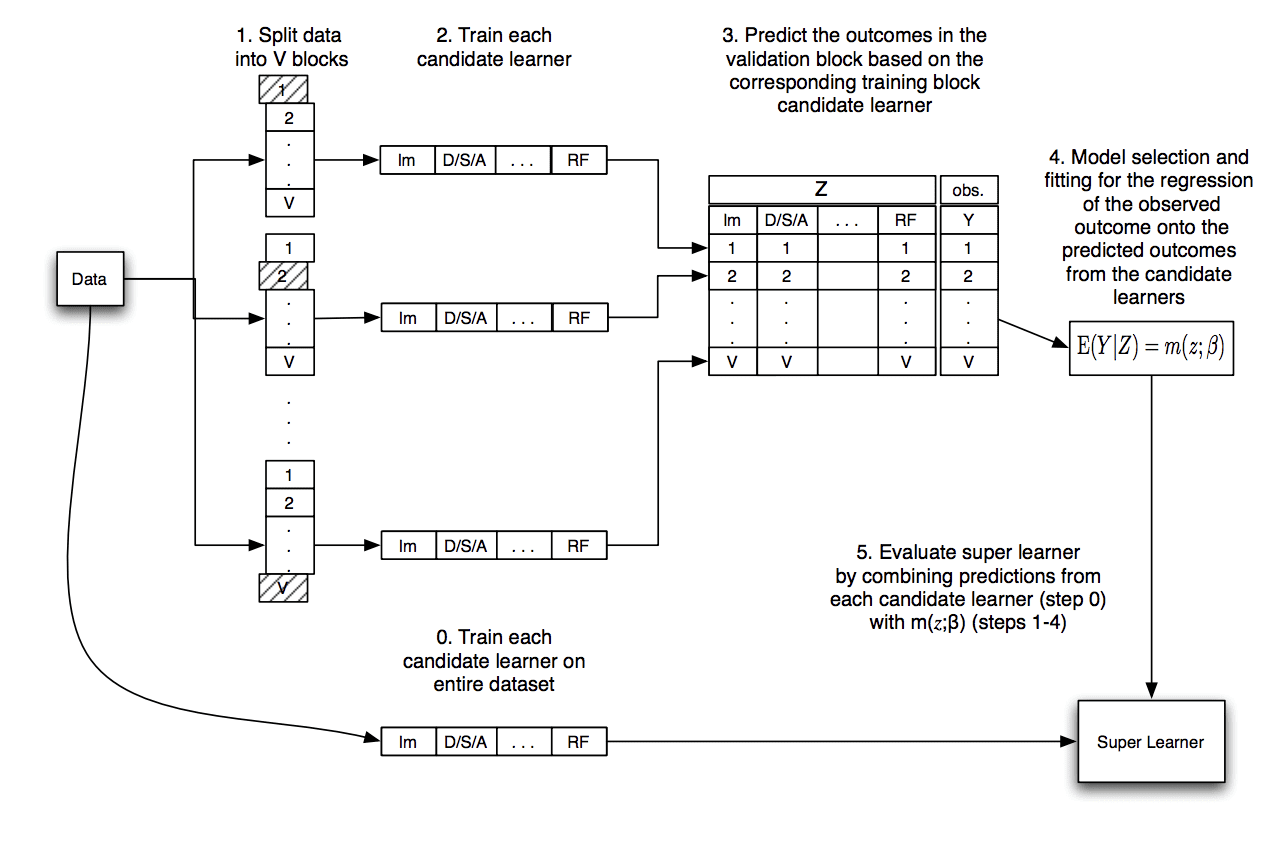
\includegraphics[width=\textwidth]{./Figures/sup-learn.jpg}
\end{figure}

\end{frame}

\begin{frame}{The Super Learner flow diagram}

\vspace*{0.25em}\begin{tikzpicture}
	\tikzset{help lines/.append style=pink}
%	\draw [help lines] (-5,-4) grid (6,4); \node[draw,circle,red] at (0,0) {};

	% start with full training data
	\node[right,font=\small] (data) at (-5,0) {$\mathcal{D}=\set{(x_i,y_i)}_1^N$};

	% path 1: full training data
	\node[draw,rectangle,minimum width=2cm,minimum height=0.5cm,font=\small] (full) at (-1,2) {$\hat{\phi}_1, \hat{\phi}_2,\dots,\hat{\phi}_K$};
	\begingroup\linespread{0.9}\node[font=\footnotesize,text centered,text width=2.5cm] at ($(full)+(0,0.8)$) {strong learners on full $\mathcal{D}$, $\hat{\phi}_k(\boldsymbol{X})$};\endgroup
	\begingroup\linespread{0.9}\draw[-latex,bend left,thick] (data.north) to node[font=\footnotesize,above left,text centered,text width=1.5cm] {learners prediction} (full.west);\endgroup

	% path 2: cross-validation for weights
	\node[font=\footnotesize,below] (cross) at (0,-1.5) {
		$\begin{array}{cccc|c}
			\hat{\phi}_1 & \hat{\phi}_2 &\dots & \hat{\phi}_K & Y \\
			1 & 1 & \dots & 1 & 1 \\
			2 & 2 & \dots & 2 & 2 \\
			\vdots & \vdots & \ddots & \vdots & \vdots \\
			V & V & \dots & V & V
		\end{array}$
	};
	\begingroup\linespread{0.95}\node[font=\footnotesize,text centered,text width=3cm] at ($(cross.north)+(0,0.4)$) {cross-validation $\hat{\phi}_{k,T(\nu)}(\boldsymbol{X}_{V(\nu)})$};\endgroup
	\begingroup\linespread{0.9}\draw[-latex,thick,bend right] (data.south) to node[font=\footnotesize,below left,text centered,text width=1.5cm] {prediction weights} (cross);\endgroup

	% end with prediction
	\node[left] (pred) at (6,0) {$\hat{\phi}_{\text{SL}}=\sum_{k=1}^K{\color{mLightGreen}\hat{\alpha}_k}{\color{mLightBrown}\hat{\phi}_k}$};
	\draw[-latex,bend left,thick,mLightBrown] (full.east) to (pred);
%	\draw[-latex,thick,bend right,mLightGreen] (cross) to node[font=\scriptsize,below right,mDarkTeal] {$\argmin_\alpha\sum_{i=1}^NL(Y_i,m(z_i\rvert\alpha))$} (pred);
	\draw[-latex,thick,bend right,mLightGreen] (cross) to (pred);
	\node[font=\scriptsize] (alph) at (4,3.3) {$\hat{\alpha}=\argmin_\alpha\sum_{i=1}^NL(Y_i,m(z_i\rvert\alpha))$};
	\node[font=\scriptsize] at ($(alph)+(0,-0.55)$) {$m(z\rvert\alpha)=\sum_{k=1}^K\alpha_k\hat{\phi}_{k,T(\nu)}\bigl(\boldsymbol{X}_{V(\nu)}\bigr)$};
\end{tikzpicture}

\end{frame}

\begin{frame}{Super learner in practice}

\begin{columns}[T]
\begin{column}{0.5\textwidth}
Package \texttt{SuperLearner}
\end{column}
\begin{column}{0.5\textwidth}
% una sorta di variable importance ma per i pesi degli strong learners

\end{column}
\end{columns}

\end{frame}

% ------------------------------- %

\begin{frame}{Scores}

% il super learner riesce a prendere il meglio da questi modelli??

\begin{table}
\sisetup{round-mode=places}
\resizebox{0.9\textwidth}{!}{
\vspace*{-1em}\begin{tabular}{lS[round-precision=4]S[round-precision=4]}
\toprule
Model & {Train score} & {Test score} \\
\midrule
CART & 0. & 0. \\
Random forest & 0. & 0. \\
AdaBoost & 0. & 0. \\
Super learner & 0. & 0. \\
\bottomrule
\end{tabular}}
\end{table}

\end{frame}








